%!TEX root = ../doc.tex
\chapter{Konzept}
\label{sec:konzept}

Aus den Anforderungen ist klar ersichtlich dass eine eigene Benutzeroberfläche entwickelt werden soll, welche über die Programmierschnittstelle von LoBo kommunizieren soll. Die nicht funktionelle Anforderung NFREQ-001 verlangt eine Web Browser kompatible Benutzeroberfläche und disqualifiziert eine zu installierende Desktop Client Anwendung. Trotz der Limitierung der Lösungsmöglichkeiten, bleiben bei der Entwicklung einer Benutzeroberfläche im Web viele Fragen offen. Im folgenden werden die Technologie- sowie Architekturentscheidungen vorgestellt und begründet.

\section{Web Modell}
Traditionelle Websites bestehen aus mehreren \textit{Hyper Text Markup Language} (HTML) Seiten und liefern diese, wenn der Client sie anfordert aus. Es gibt verschiedene Programmiersprachen welche es erlauben zum Zeitpunkt des Aufrufs, Code welcher in diesen HTML Seiten vorhanden ist zu interpretieren und des entsprechende Resultat auszuliefern. \textit{PHP Hypertext Preprocessor}\footnote{Offizielle Website von PHP: \url{http://php.net/}} (PHP) ist eine der bekanntesten Programmiersprachen. Aber auch Python bietet mit dem Framework \textit{Django}\footnote{Offizielle Website von Django: \url{https://www.djangoproject.com}} eine ähnliche Funktionalität an. Mit der zunehmende Möglichkeiten im Web sowie der immer grösseren Komplexität wurden andere Modelle für das Web entwickelt. Mit der offiziellen Spezifikation des \textit{XMLHttpRequest Object} am 5. April 2006\citep[]{w3cXMLHttpRequest} und dessen Einsatz von Google in Webapplikationen wie Gmail und Google Maps, wurde die Entwicklung von \textit{Single-page application} (SPA) ermöglicht. Mit \textit{XMLHttpRequest} ist es möglich nach dem Laden der Website eine Anfrage an den Server zu schicken ohne dabei die Gesamte HTML Seite neu zu laden. Für die Ausführung dieser \textit{XMLHttpRequest} Anfragen wird eine clientseitige Skriptsprache benötigt. Trotz vereinzelten Alternativen ist JavaScript der Standard bei den browserfähigen clientseitigen Skriptsprachen. Dies ist mitunter auch ein Grund warum SPA Webseiten mit JavaScript erstellt werden. In den Abbildungen  \ref{fig:requestHtml} und \ref{fig:requestXHtml} \footnote{Bilder von \url{https://blog.4psa.com/an-intro-into-single-page-applications-spa/}} ist der Unterschied zwischen einer konventionellen Website und einer SPA veranschaulicht.

\begin{figure}[ht]
	\centering
  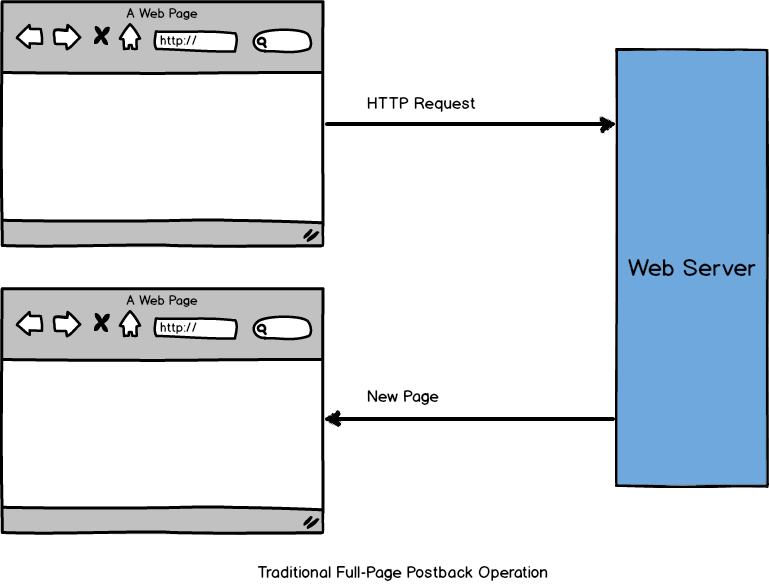
\includegraphics[width=0.88\textwidth]{images/requestHtml.png}
	\caption{Visualisierung einer Anfrage in einer konventionellen Webseite}
	\label{fig:requestHtml}
\end{figure}

\begin{figure}[ht]
	\centering
  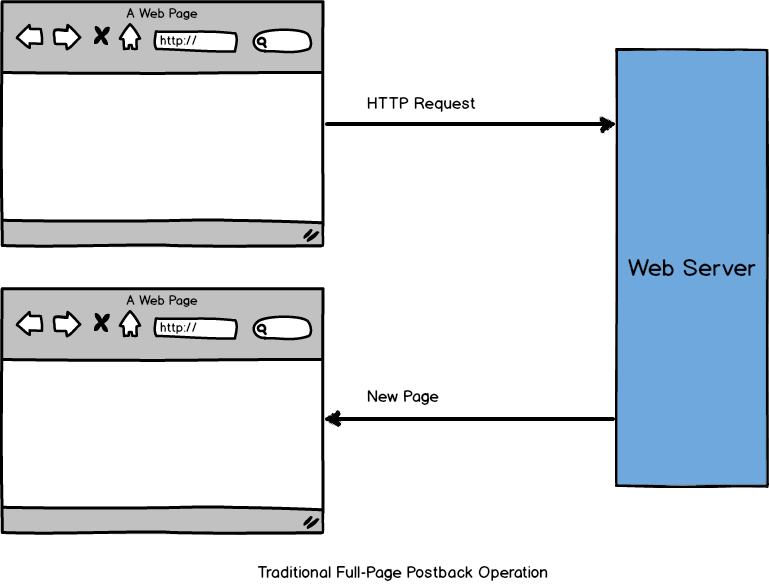
\includegraphics[width=0.88\textwidth]{images/requestHtml.png}
	\caption{Visualisierung einer Anfrage in einer Single-page Applikation}
	\label{fig:requestXHtml}
\end{figure}


\subsection{Single-page application}
\textit{Single-page application} (SPA) haben viele Vorteile gegenüber traditionellen Webseiten. Die Gesamte Webseite kann mit wenigen Anfrage an den Server geladen werden. Im wesentlichen werden nur drei Anfragen (1. HTML Seite, 2. Cascading Style Sheets (CSS), 3. JavaScript) benötigt. Alle weiteren Daten wie z.B. Benutzerdaten aus der Datenbank werden asynchron mit einer \textit{XMLHttpRequest} Anfrage, während die Webseite im Browser aufgebaut wird, geladen. Dies hat den Vorteil dass die Webseite bedeutend schneller geladen wird und trägt damit zur Benutzerfreundlichkeit bei. Im folgende ist eine nicht abgeschlossene Liste mit den Vorteilen von SPA.
\begin{description}
	\item[Entlastung] Die Benutzeroberfläche wird komplett im Browser erstellt und benötigt dafür keine Ressourcen vom Server.
	\item[Entkopplung] Daten und Businesslogik sind nicht mehr an die Visuellen Elemente gebunden.
	\item[Performant] Single-page Applikationen verwalten ihren eigenen Status und benötigten dafür weniger Informationen vom Server.
\end{description}
SPA setzten voraus dass der Server ein definierte Schnittstelle besitzt über welche Daten geladen bzw. geschrieben werden können. Dies hat zusätzlich der Vorteil, dass auch Applikationen anderer Plattformen wie z.B. Android oder iOS auf diese Schnittstellen zugreifen können.
\newline{}
Ein grosser Nachteil von Single-Page Applikationen ist die Lesbarkeit des auszuführenden Codes. JavaScript ist eine Skriptsprache welche zur Laufzeit interpretiert und ausgeführt wird. Dies bedeutet dass der gesamte Code im Browser vorhanden ist und für den Benutzer lesbar ist. Es gibt Werkzeuge welche diesen Code versuchen unleserlich zu machen in dem Variablen umbenennt und Leerzeichen entfernt werden, aber mit Energie und Geduld kann auch dies wieder lesbar gemacht werden.

\subsection{Mini-Backend}
Für die Auslieferung der \textit{Single-page application} wird nur ein Webserver wie z.B. Apache\footnote{Apache ist ein weitverbreiteter opensource Webserver \url{https://httpd.apache.org/}} oder Nginx benötigt. Die SPA kann aber auch von einem Webserver ausgeliefert werden, welcher eigene Logik besitzt. Im Rahmen dieser Bachelorarbeit nenne ich die Benutzung eines Webservers mit eigener Logik Mini-Backend. Es existieren mehrere Plattformen in verschiedenen Programmiersprachen mit welchen die Entwicklung eines Mini-Backend möglich wäre.  Node.js\footnote{Node.js ist eine Serverseitige Plattform \url{https://nodejs.org}} ist eine serverseitige Plattform welche auf JavaScript basiert und die Möglichkeit bietet Webseiten auszuliefern und eigene Logik auszuführen. Diese Logik bzw. dieser Code befindet sich immer auf dem Server und kann von den Benutzer nicht gelesen werden. Node.js kann die gesamte Businesslogik eines Projektes beinhalten oder aber nur Webanfragen weiterleiten

\subsection{Fazit}
Obwohl die Logik für die zu entwickelnde Benutzeroberfläche ausschliesslich in der SPA ausgeführt werden könnte, hat der Einsatz eines sogenannten Mini Backends erhebliche Vorteile. LoBo benutzt für die Authentifizierung einen Schlüssel mit welchem alle Anfragen \textit{gehasht} werden müssen. Der Entstandene Hash wird im Header jeder Anfrage mitgeschickt. Dadurch kann LoBo die Authenzität und Integrität der Anfragen sicher stellen. Dieses hashing könnte in der SPA geschehen, hat jedoch den Nachteil, dass der Schlüssel von den Benutzer ausgelesen werden kann. Zusätzlich vereinfacht der Einsatz eines Mini-Backend die Skalierung. Weil die Mini-Backends nicht auf eine Datenbank zugreifen, können einfach mehrere Instanzen gestartet werden und ein zusätzlicher Webserver verteilt die Anfragen auf die verfügbaren Instanzen. Die Mini-Backends können auch mit verschiedenen LoBo Systemen kommunizieren. Dies verhindert einen Flaschenhals bei einem Anstieg der Benutzerzahlen. Im Rahmen dieser Bachelorarbeit wird eine Single-page Applikation mit JavaScript entwickelt und ein Mini-Backend welches auf Node.js basiert. Node.js wurde ausgewählt weil es in der gleichen Sprache programmiert wird, wie die SPA und dadurch einige Vorteile für den Entwickler bietet. Der Entwickler braucht während der Entwicklung nicht den Kontext zu wechseln und kann unter Umständen die gleichen Ressourcen für die SPA wie auch das Mini-Backend verwenden.

\section{JavaScript}
JavaScript ist eine zurzeit populäre Programmiersprachen welche zu einem grossen Teil für dynamischen Aspekte einer Webseite verantwortlich ist aber auch Serverseitig zum Einsatz kommt. Obwohl während den Anfängen von JavaScript mehrere Interpretationen der Sprache existierten, ist JavaScript heute der einzige Dialekt welcher auf der EcmaScript Spezifikation basiert und interpretiert wird. JavaScript wird von allen grossen Browsern mit ihren jeweiligen Implementationen unterstützt. Im folgenden eine Liste der JavaScript Engines der bekanntesten Browsers\footnote{Liste von Wikipedia \url{https://en.wikipedia.org/wiki/ECMAScript}}.
\begin{description}
	\item[SpiderMonkey] wird von Mozilla für den Browser Firefox entwickelt.
	\item[V8] wird von Google für den Browser Chrome entwickelt.
	\item[JavaScriptCore] wird von Apple für den Browser Safari entwickelt.
	\item[Chakra] wird von Microsoft für den Browser Edge entwickelt.
\end{description}
V8 von Google wird unter anderem auch für Node.js verwendet welches im Rahmen dieser Bachelorarbeit für das Mini-Backend verwendet wird.

\subsection{ES2015}
Die Sprache hat im Juni 2015 eine lang erwartet neue Version bekommen. Ecma International\footnote{European Computer Manufacturers Association \url{http://www.ecma-international.org/}} welche die Spezifikationen für die Programmiersprache JavaScript schriebt, hat die Version EcmaScript 2015 veröffentlicht und damit der Sprache einige neue Funktionen verleihen. Mit EcmaScript 2015 (ES2015) können Klassen erstellt werden und mit einem Module System Klassen, Objekte, Funktionen und Variablen exportiert wie auch importiert werden. Dank dieser Erneuerung ist es bedeutend einfacher JavaScript Code zu unterhalten und pflegen. Er kann in verschiedene Module unterteilt werden und ist dadurch auch besser lesbar. Einige der Erneuerungen machen auch Helfer Bibliotheken wie \textit{underscore.js} oder \textit{jquery} überflüssig, was wiederum zur Performanz beiträgt.

\subsection{Backend Framework}
Für Node.js existieren mehrere Webserver Frameworks welche für den Einsatz im Rahmen dieser Bachelorarbeit eingesetzt werden können. 3 Populäre Frameworks sind Express.js\footnote{Web Framework für Node.js \url{http://expressjs.com/}}, Koa.js\footnote{Web Frameork für Node.js \url{http://koajs.com/}} und hapi.js\footnote{Web Framework für Node.js \url{http://hapijs.com/}}. Express.js jedoch ist das populärste Framework und findet auf Github die grösste Unterstützung.\citep[]{nodejsframeworks}. Die Entwicklung der Mini-Backends benötigt keine aussergewöhnlichen Anforderungen und hat mit Express.js alle Ansprüche abgedeckt.

\subsection{Frontend Framework}
In JavaScript existieren unzählige Frameworks welche etliche Anwendungsfälle unterstützten können. Obwohl eine Single-Page Applikation auch ohne Framework und Helfer Bibliothek entwickelt werden kann, können Frameworks zur stabilität und erfolg der Webseite beitragen. Frameworks wie Angular\footnote{Javascript Framework von Google \url{https://angularjs.org/}} und Ember.js\footnote{Javascript Framework aus der OpenSource Gemeinschaft \url{http://emberjs.com/}} unterstützen die Entwicklung einer \textit{Model View Controller} (MVC) SPA erheblich. Angular stellt z.B. einen Service (\textit{\$resource}) zur Verfügung mit welchem alle \textit{XMLHttpRequest} Anfragen ausgeführt werden können. Die Handhabung im Falle eines Fehlers kann zentral implementiert werden und auch die Transformation von Empfangen sowie zu Versendenden Daten kann mit dem Service verwaltet werden. In Ember.js wird eine Datenverwaltungs Komponente zur Verfügung gestellt, welche die gesamte Synchronisation der Daten mit einem Backend übernimmt. Sofern das Backend eine standardisierte JSON REST\footnote{REST steht für \textit{Representational State Transfer} und bezeichnet ein Programmierparadigma} Programmierschnittstelle besitzt, kann diese Synchronisation, welche Daten erstellt, bearbeitet, lädt und löscht, mit wenigen Zeilen Code implementiert werden. Diese Beispiele sind nur vereinzelte Einblick in die Möglichkeiten der Frameworks. Frameworks bringen aber auch Nachteile mit sich, sobald ein Anwendungsfall implementiert werden soll, welcher nicht dem Framework entspricht, kann es kompliziert und Fehleranfällig werden.
\newline{}
Ein relativ neues JavaScript Framework ist \textit{React}\footnote{JavaScript Framework von Facebook \url{https://facebook.github.io/react/}} welches von Facebook entwickelt wird. React setzt im Gegensatz zu MVC Frameworks eine andere Philosophie um. Zum einen wird in React mit Komponenten, welche wiederum Subkomponenten beinhalten können, gearbeitet. Zum anderen wird das Programmierparadigma \textit{Data Down, Actions up} umgesetzt. In diesem Programmierparadigma wird den Komponenten die Benötigten Daten übergeben und die Komponenten rufen eine Methode auf welche die bearbeitet Daten zurück gibt. Zusätzlich werden die \textit{Templates} welche benötigt werden für die visuelle Repräsentation der Komponenten nicht wie üblich in HTML geschrieben sonder in JSX\footnote{JSX steht für \textit{JavaScript Syntax extension} und erlaubt das Schreiben von HTML in JavaScript} womit der gesamte Code einer Komponente in der gleichen Datei geschrieben werden kann. Auch von Facebook stammt die Applikations Architektur \textit{Flux}. Flux besteht aus hauptsächlich aus einem \textit{Dispatcher}, \textit{Store} und den \textit{Views} und baut auf einigen wenigen Prinzipien auf welche in der folgenden Liste erklärt werden.
\begin{description}
	\item[Unidirektionaler Datenfluss] Daten fliesen immer in eine Richtung. Jede Änderung der Daten findet über eine Aktion statt.
	\item[Klare Trennung der Kontrolle] Die Kontrolle über die Daten befindet sich in den \textit{Stores} und diese können von Aussen nicht verändert werden.
	\item[Zentralisierter Dispatcher] Es existiert nur ein \textit{Dispatcher}, welcher alle \textit{Stores} über eine neu Aktion informiert. Dadurch wird garantiert, dass immer nur eine Aktion aufs mal ausgeführt wird.
\end{description}
Flux und die Prinzipien sind in der Abbildung \ref{fig:flux} dargestellt.

\begin{figure}[ht]
	\centering
  
\includegraphics[width=0.88\textwidth]{images/flux.png}
	\caption{Darstellung des Programmierparadigma Flux}
	\label{fig:flux}
\end{figure}
Flux und React können kombiniert werden und ergeben dadurch ein stabiles, modernes und Fehlerarmes JavaScript Framework.

\subsection{Fazit}
Aus den Anforderungen in Kapitel \ref{sec:anforderungsanalyse} wird klar, dass die gleichen Eingabemasken an verschiedenen Stellen zum Einsatz kommen. Die Eingabe einer Adresse wird gleich in mehreren Anforderungen benötigt. Für diese Anforderung spricht ein Framework wie React, welches diese Eingabemasken als Komponenten einmal implementiert und an verschiedene Stellen zu Verfügung stellt. Auch der Aufbau einer Schritt für Schritt Eingabe lässt sich in Komponenten und Subkomponenten praktisch umsetzten. Weil für die Erstellung eines Auftrags in LoBo einem klaren Prozess gefolgt werden muss, eignet sich der Einsatz von Flux. Mit Flux ist die gesamte Single-page Applikation weniger störungsanfällig und hat zu jedem Zeitpunkt einen klaren Zustand. Im Rahmen dieser Bachelorarbeit wird die zu erstellende Benutzeroberfläche mit React und Flux entwickelt.


\section{Architektur}

\subsection{Mini-Backend}
Das Backend hat 2 elementare Aufgaben. Das ausliefern der SPA und das bereitstellen der Schnittstelle mit welcher die SPA kommuniziert. Die SPA befindet sich in einem Verzeichnis und wird bei einem Aufruf direkt ausgeliefert. Alle Anfrage der SPA werden an eine bestimmte URL gesendet, welche mit der Entsprechenden Antwort oder einem Fehler antwortet. Das Mini-Backend soll aber nicht nur die Anfragen von der SPA an LoBo weiterleiten sonder auch die Komplexität gewisser Prozessabläufe vereinfachen. Obwohl LoBo viele Schnittstellenendpunkte zur Verfügung stellt, werden für gewisse Funktionen mehrere Anfragen benötigt. Für Die Abfrage ob eine bestimmte Strassenadresse in einem Gebiet liegt, welches von Imagine Cargo versorgt wird, werden 3 Anfragen an LoBo benötigt. Zuerst muss in LoBo ein neuer Auftrag erstellt werden, mit dem dadurch gewonnen Auftragstoken muss eine Adresse hinzugefügt werden. Zuletzt muss eine Anfrage gestellt werden, welche überprüft ob der Auftrag konform ist. Die Fehlermeldung dieser Anfrage bestimmt ob die Adresse in einem Versorgungsgebiet von Imagine Crago liegt. Der gesamte Ablauf ist in der Abbildung \ref{fig:addressverify} grafisch dargestellt. Darin ist zu sehen wie viel Arbeit vom Mini-Backend gehandhabt wird.

\begin{figure}[ht]
	\centering
  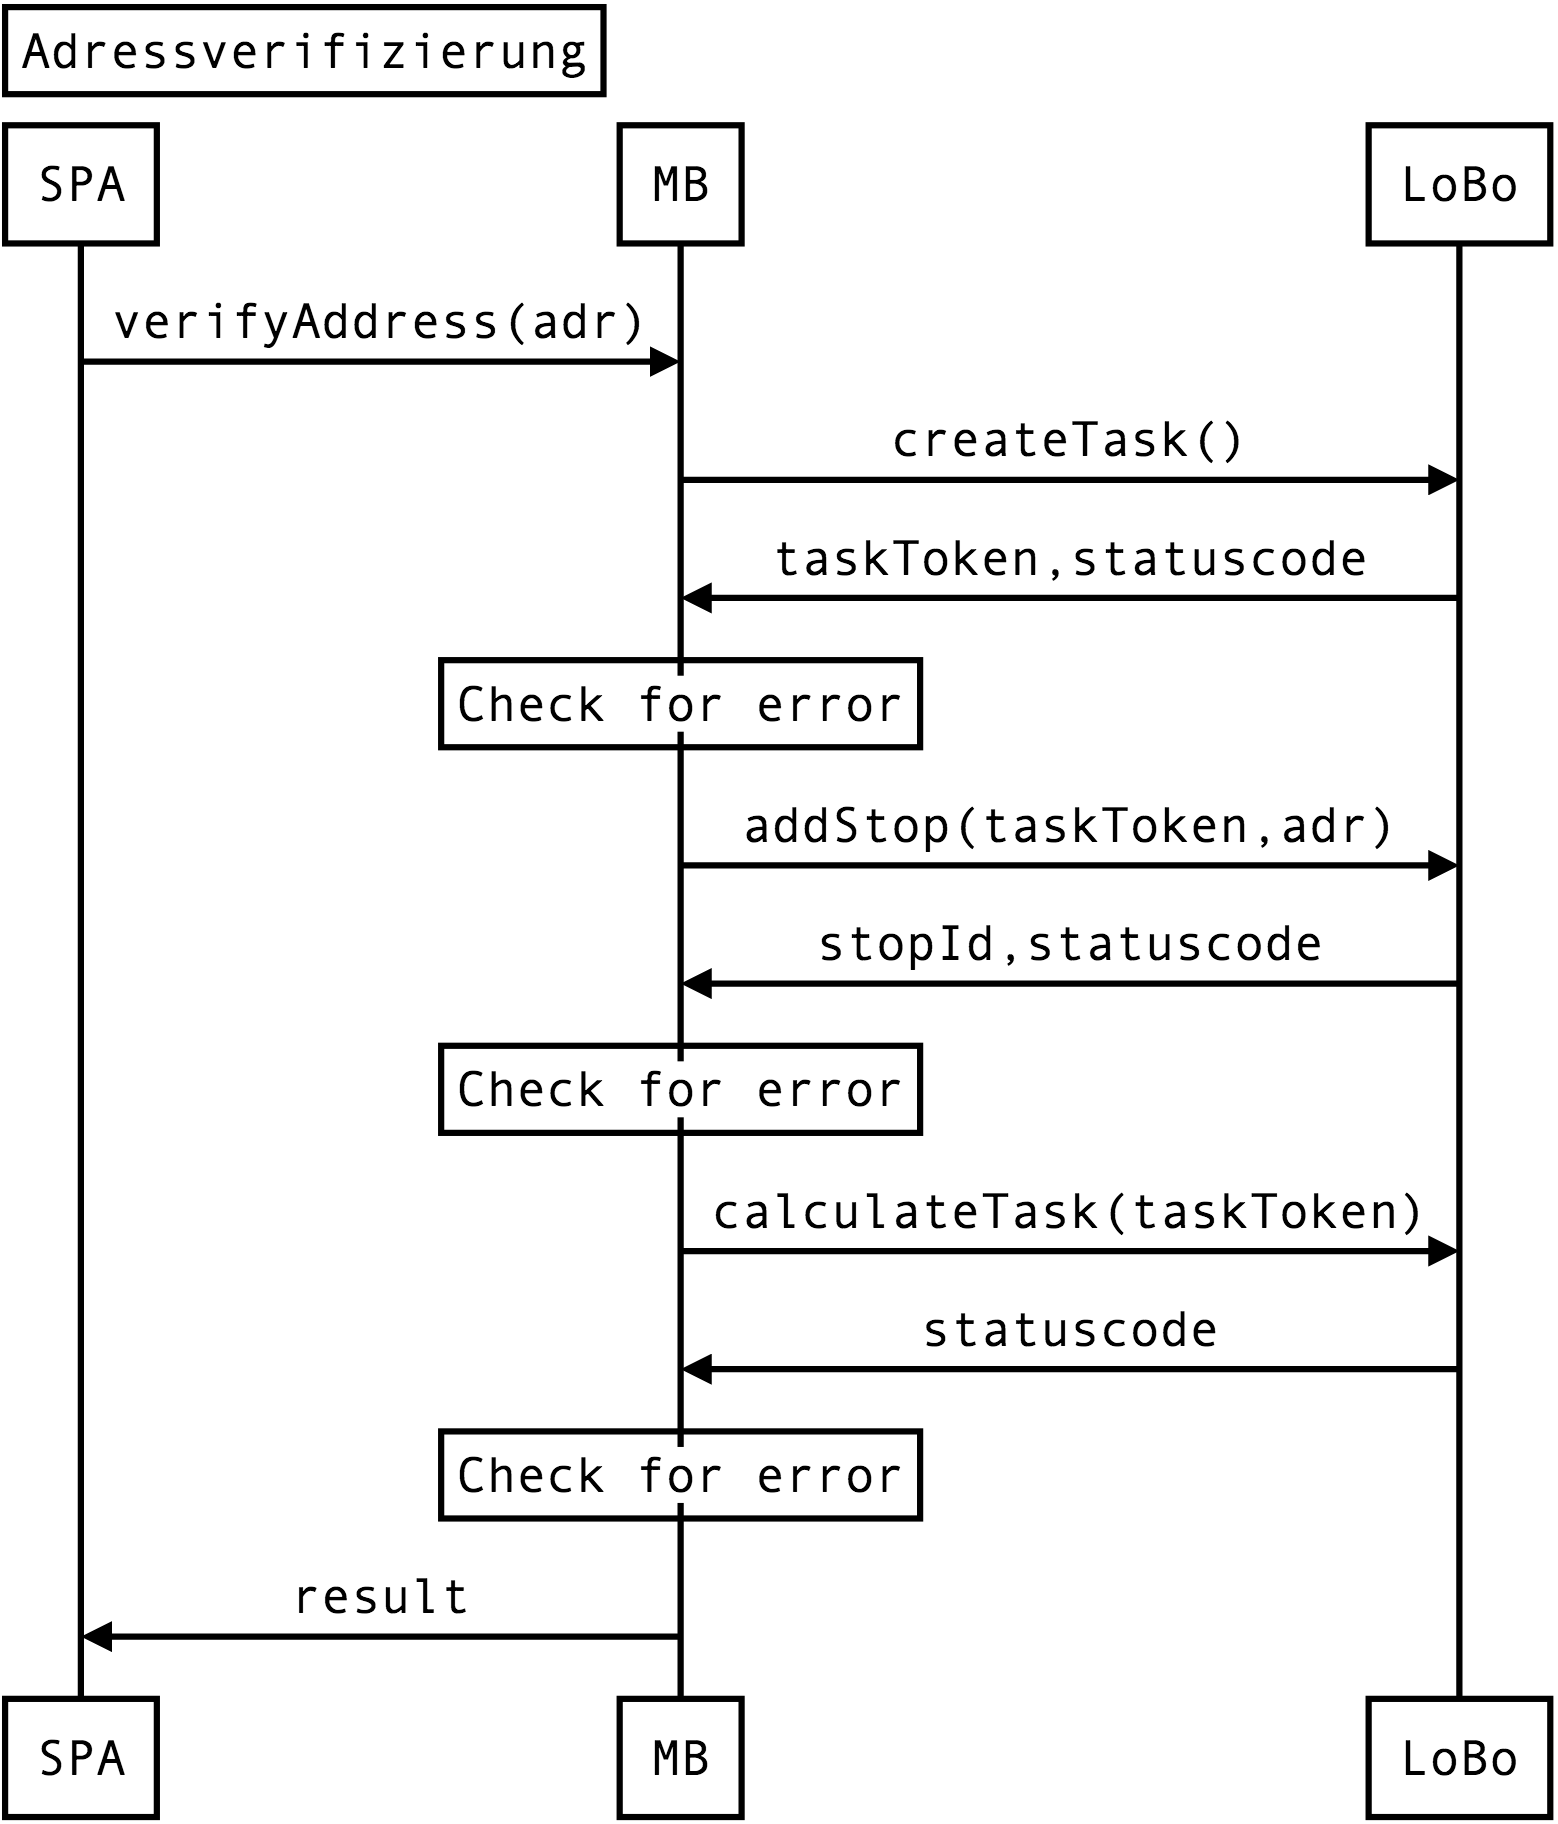
\includegraphics[width=0.88\textwidth]{images/addressverify.png}
	\caption{Darstellung des Prozesses zur Verifizierung einer Adresse}
	\label{fig:addressverify}
\end{figure}

Somit braucht das Mini-Backend nur die Schnittstellenendpunkte zur Verfügung zu stellen, welche auch zwingend von der SPA gebraucht werden. Diese Schnittstellenendpunkte sind in der folgende Liste aufgeführt und beschrieben.

\begin{description}
	\item[createtask] erstellt in Lobo einen neuen Auftrag und übergibt den \textit{tasktoken} an die SPA für alle weiteren anfragen.
	\item[verifyaddress] überprüft in einem temporären Auftrag ob die Adresse im Versorgungsgebiet liegt
	\item[addstop] fügt dem Auftrag eine Adresse hinzu.
	\item[compiletask] überprüft ob dem Auftrag noch weitere Stops (z.B. Bahnhöfe) hinzugefügt werden müssen-
	\item[updatestopinfo] fügt Informationen (z.B. Kontaktpersonen) den einzelnen Adressen hinzu.
	\item[updatestoptime] fügt die Abfahrts- und Ankunftszeit den Stops hinzu.
	\item[updatereftime] erneuert die Uhrzeit um welcher der Auftrag gestartet wird.
	\item[connections] lädt alle Verbindungen zwischen 2 Städten um eine gewisse Uhrzeit.
	\item[ordertask] finalisiert den Auftrag
\end{description}


Error handling wenn möglich nur im Backend.

\subsection{Frontend}
Alle actions wie adresse auto complete, update stop info, update task info in komponenten. können in Steps und Advanced tour wiederverwendet werden. Steps sind auch wieder komponenten welche die anderen komponenten weiderverwenden.



\section{Schnitstellen}
Lobo -> Lobo
Addresse Auto Complete -> Google Maps and Open street maps
Sbb times -> opendata.ch


\section{Bibliotheken}
%http://iso4app.net/ für die polygone
%https://github.com/tmpvar/polygon.js
%https://www.npmjs.com/package/vec2


%https://www.smashingmagazine.com/2016/06/an-introduction-to-redux/?utm_source=javascriptweekly&utm_medium=email








